\documentclass[a4paper]{article}


\usepackage{xspace}
\usepackage{a4wide}
\usepackage{hyperref}
\usepackage{amsmath}
\usepackage{graphicx}
\usepackage{enumerate}
\usepackage{verbatim}
\usepackage{listings}
\lstset{language=Haskell, basicstyle=\small}
\usepackage{amsfonts}
\usepackage{pifont}
\newcommand{\tickYes}{\checkmark}
\newcommand{\tickNo}{\hspace{1pt}\ding{55}}
\newcommand{\ar}{Archery\xspace}
\newcommand{\re}{Reo\xspace}
\newcommand{\mcrl}{$\mu$CRL2\xspace}

\hypersetup{
    %bookmarks=true,         % show bookmarks bar?
    unicode=false,          % non-Latin characters in Acrobat’s bookmarks
    pdftoolbar=true,        % show Acrobat’s toolbar?
    pdfmenubar=true,        % show Acrobat’s menu?
    pdffitwindow=false,     % window fit to page when opened
    pdfstartview={FitP},    % fits the page to the window?
    pdftitle={Modeling in \ar and \re},    % title
    pdfauthor={Jorge Cunha Mendes and Paul van der Walt},     % author
    pdfsubject={Model Checking},   % subject of the document
    pdfcreator={Jorge Cunha Mendes and Paul van der Walt},   % creator of the document
    pdfproducer={}, % producer of the document
    pdfkeywords=
        {\re}
        {\ar}
        {Modeling}, % list of keywords
    pdfnewwindow=true, % links in new window
    colorlinks=true,   % false: boxed links; true: colored links
    linkcolor=blue,    % color of internal links
    citecolor=blue,    % color of links to bibliography
    filecolor=blue,    % color of file links
    urlcolor=blue      % color of external links
}

\author{Jorge Mendes \and Paul van der Walt}
\date{\today}
\title{Modeling in \ar and \re}
\begin{document}

\maketitle

%
% Intro
%
\section{Introduction}

This project aims to model a system using two distinct frameworks, namely \ar
and \re, and to compare both approaches.

\ar is a modeling language developed at the University of Minho, which is designed
to be a higher-level modeling language for software architectures. There is a translator
that converts \ar models to \mcrl, making it possible to use a set of tools that work with
\mcrl to check properties about the developed models and also to simulate and visualize them.

\re is a research activity of the SEN3 research group at the CWI, in the
Netherlands. It provides a paradigm for composition of distributed software
components and services based on the notion of mobile channels.
From this research activity, resulted the \re coordination language and the
Extensible Coordination Tools (ECT) which are a set of plug-ins for the Eclipse
platform to deal with the coordination language.

The chosen system is a dynamically adjustable cluster of servers for a news
agency. Depending on the load of the system, it should add or remove servers
from the cluster. If the load is too high with all the servers available for
the cluster, then the servers should respond without media content, i.e., they
should respond with only the text of the requested page (media mode vs. text
mode).

%
% The problem
%
%\section{The Problem}
%
%The problem was to model a news website, which consists of users, a load
%balancer, and a number of servers. There is some maximum $M$ of servers, and
%when the load balancer detects that the network is busy, servers can dynamically
%be added to the pool up to this maximum $M$. A server can also answer in media
%or text mode, depending on the load conditions. The aim is to guarantee that all
%requests will be serviced within a certain time limit $x$, by adding servers
%when necessary, spreading the load evenly, and switching down to text-mode when
%the servers are too busy. A server can respond to a given number of requests per
%minute in media mode, and $asdf$ per minute in text mode (with $asdf<asdf$

% XYZ News is proud to be the reliable online news agency to first provide information in different formats to its audience. Their journalists arrive where news take place and prepare text, images and videos to be put online. However, their reputation has a price. Whenever an important event takes place, the website receives massive amounts of requests for a short period of time. XYZ applies two tactics to manage these peaks. The first is to dinamically add up to N web servers to the cluster and the second is to provide only text content in articles. Then, a server can be attending requests in either a full-media or a text-only mode. The first tactic is used until there are no more available servers. Then, the second is applied. XYZ board wants that every request is answered, and if possible, in less than n (n > m) miliseconds. They know that a server can respond in less than m miliseconds up to R simultaneous requests in full-media mode, and up to Q in the text-only one.

%
% Approach
%
\section{Approach}

There are several possible approaches to model the news system. The ones that we
thought of are all based on the same idea: clients, servers and a load balancer. The
functionalities and arrangement of these elements for each architecture is what
changes between the approaches.

In the first approach, we can make the clients and the servers communicate with
each other
directly. Also, the servers communicate with the load balancer to
know if they should accept more requests and which mode (full-media or
text-only) should be used to provide the response. The architecture of this
approach is depicted in Figure \ref{fig:cslb}. However, this approach needs
a lot of connections from the clients to servers.

\begin{figure}[htb]
	\begin{center}
		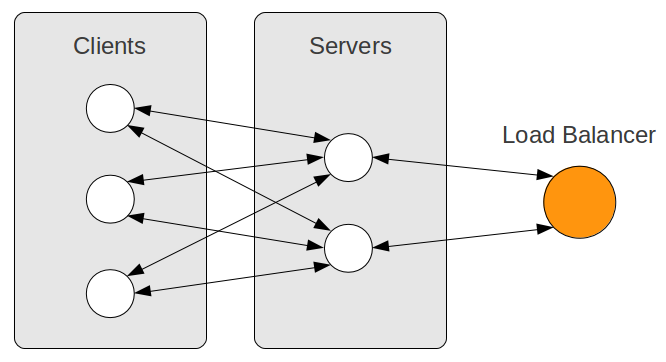
\includegraphics[width=0.5\textwidth]{images/c_s_lb.png}
	\end{center}
	\caption{Client $\leftrightarrow$ Server $\leftrightarrow$ Load balancer }
	\label{fig:cslb}
\end{figure}

The second approach, depicted in Figure \ref{fig:clbs}, is the one that we
tried to implement, and provides a single point of communication between the
clients and the servers. It results in less channels for communication, but the
load balancer needs to be aware of the clients identification to route the
requests/reponses correctly.

\begin{figure}[htb]
	\begin{center}
		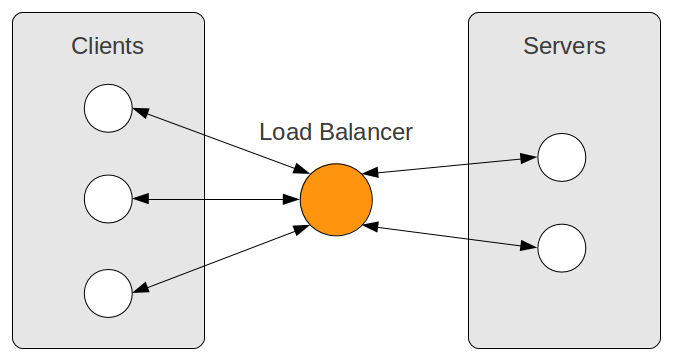
\includegraphics[width=0.5\textwidth]{images/c_lb_s.png}
	\end{center}
	\caption{Client $\leftrightarrow$ Load balancer  $\leftrightarrow$ Server }
	\label{fig:clbs}
\end{figure}

% TODO describe Archery approach(es)

\subsection{\ar Approach}

The basic approaches described above were modeled in \ar. However, due to some
limitations in \ar (or the translator), we've not been able to create a full
model of the system.

We first tried the approach described in Figure \ref{fig:cslb}, but we hadn't
enough knowledge at the time about out to implement the identification of the
clients.

Then we tried the other approach (Figure \ref{fig:clbs}), which we dropped because we had to set all
the attachments by hand and that version has too many connections.

After those failed attempts, we tried again the approach from the first
attempt, but we couldn't complete it because of the language / translator
limitations.

% TODO describe Reo approach(es)

\subsection{\re Approach}

We tried a number of approaches in \re, and had varying degrees of success. The
current incarnation, and so far most successful, is using the following
architecture. In Figure \ref{fig:reo} one can see the global layout of the \re
model. We have the clients on one side, which connect to the load balancer.
There is an 'internet' entity in between which models that requests arrive at
the load balancer sequentially. The load balancer then distributes the requests
to one of the servers in the pool. Unfortunately, some of the things we would
have liked to model weren't possible using \re. For example, we have two
versions of the load balancer, one which nondeterministically distributes the
request to one of the servers which is in a suitable state to receive a request,
and the other version which distributes the request in a round-robin fashion.
Both have disadvantages, since in the first case we're actually modeling a
'magic' load balancer, and provide no details on how this should be implemented
in real life. One way could be for the load balancer to maintain a worklist of
unanswered requests, which servers could poll as soon as they have time. This is
unrealistic, however, since in real life the servers usually don't have control
over when requests arrive. The second method (round robin) has a pitfall which
is more related to our lack of experience with \re. The problem is that if it is a
given servers turn, but that server is still busy servicing the last request,
the load balancer blocks until the server is free again. This is undesirable,
since another server might be idle. It would, however, be easier to implement
this solution in real life.

In the actual \re model, servers are represented by two components. The one
component just receives the request and passes it along to the actual server
process, but will not accept another request until the server has delivered some
response. The servers are modeled as entities with 2 FIFO's, one representing
the media mode, and the other representing text mode. In \re this makes no
difference, but if one exports the model to \mcrl, probably a different delay
per channel could be
implemented there.

The other thing that was needed, was to somehow send the server's response back
to the right client. The way this was solved in the \re model is by creating a
connector which receives all the responses and filters them. Unfortunately \re
doesn't actually know what value a given token has, even though this is
reflected in the generated \mcrl code. The result is that the filter is seen as
a pipe which may, or may not, transmit each packet, so an alternative animation
is generated each time. This is also not the way things usually work in real
life, but to keep the load balancer model simple, we chose this solution.

Also note the 'request sequencer', which just serves to collect the incoming
requests and feed them to the load balancer one at a time. This is accomplished
by a FIFO$_k$ buffer, where $k$ should be large enough to hold any number of
requests which might be incoming. In the model, only 3 buffers are used to try
and limit the state space. Also, only 3 clients and 3 servers are used, but even
this model couldn't be animated in reasonable time without simplifying it quite
drastically (removing servers and clients).

In this model, clients are modeled as a reader/writer pair, with the reader
having as many requests as the writer. In \re, this isn't sufficient to make
sure the \emph{correct} $n$ requests are received, but the framework for
checking this is present (the filters), and this could be patched up later in
\mcrl. We also don't explicitly support adding and removing servers from the
pool, but we consider an idle server as being able to turn itself off.

\begin{figure}[h]
    \begin{center}
        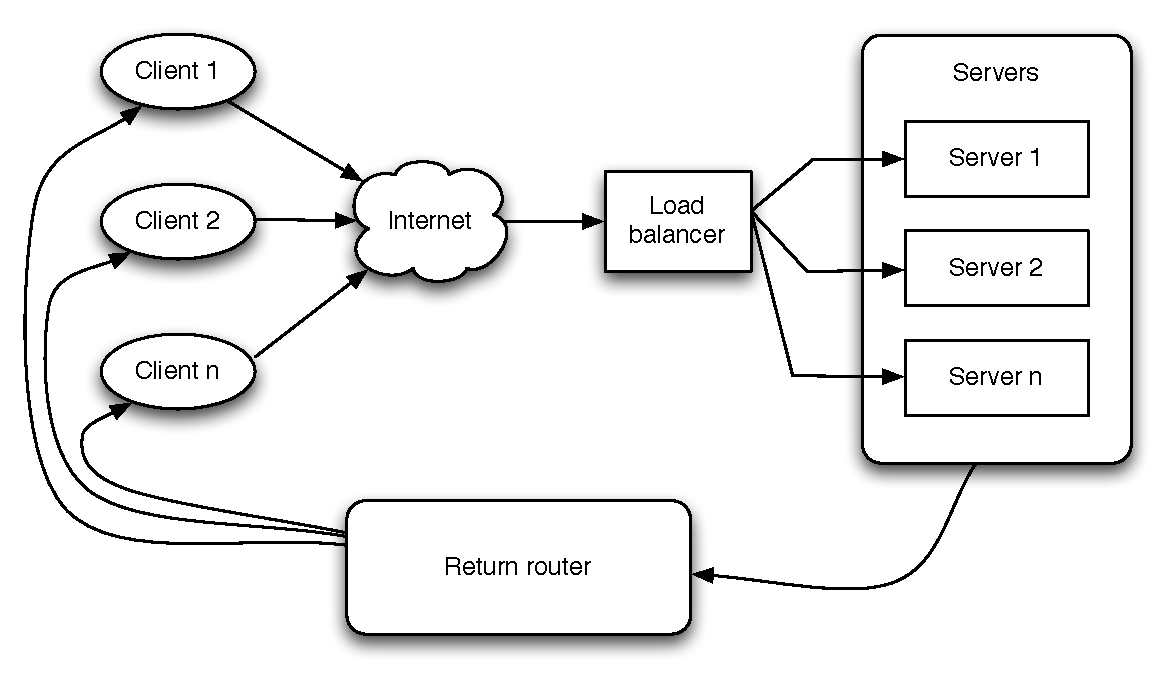
\includegraphics[width=0.8\textwidth]{images/reo-model.pdf}
    \end{center}
    \caption{Summary of the \re model.}
    \label{fig:reo}
\end{figure}

\section{\mcrl Approach}

For comparison, we also implemented a version directly in \mcrl, since we were
more familiar with this tool, and it allowed us to clarify the problem before
trying in the other tools.
%
% Archery and Reo
%
\section{Evaluating \ar and \re}

In this section we will detail the approaches we used to model the problem in
both \ar and \re, as well as design decisions and simplifications we made to the
original problem.



% Archery
\subsection{\ar}

The first small and obvious frustration with \ar is its lack of support for
comments in the model.

% Reo
\subsection{\re}


% Archery vs. Reo
\subsection{\ar vs. \re}

\ar winning\dots

%
% Conclusion
%
\section{Conclusion}
We couldn't provide a complete model in each framework, but we were able to
experiment with them and find some of their limits. However, we did not use all the
functionalities from each framework due to lack of documentation. For \re there
is some documentation, but only about the coordination language, and not about
the tools to work with the language.

\ar provides a better readability of the models code, with better organization
of it, comparing to \mcrl models. However, \ar misses some features available
in \mcrl, notably summands and paralelization, and the language or translator is
fairly limited. Also, a graphical interface would improve the development of
\ar models a lot (for example, all the connections can become quite a mess in
\ar).

% TODO no dynamic connections! Pity for dynamically adding servers. 

\re is powerful, due to the possibility of programming the components in Java,
but we didn't find a way to use those components in our model using the ECT nor
using ReoLive. Another limitation that we found in \re is the fact that it
doesn't have proper support for values like integers in the tokens using the
ECT. The graphical editor available in the ECT provides an easy to read
visualization of the model, but lacks in some basic functionalites like
copy/paste.

Both \ar and \re provide a translation to \mcrl. \re provides correct \mcrl
code whilst \ar may be translated to invalid \mcrl, probably because there is
no type check.

%Make a note about the fact that \re cannot handle values in the tokens! %todo


\appendix
\section{Full \re model}\label{app:reo}


    \begin{center}
        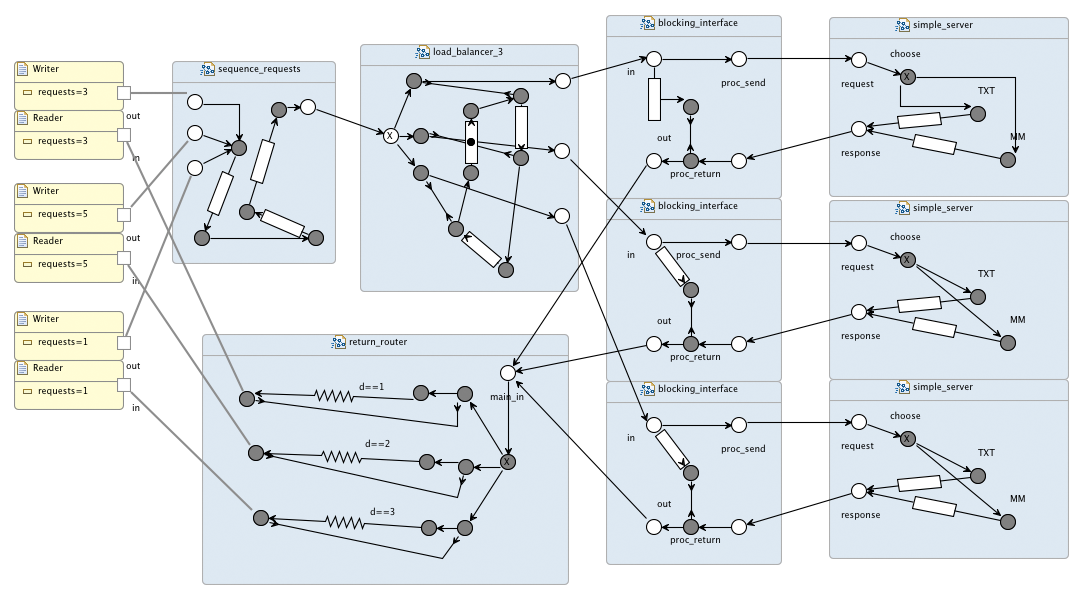
\includegraphics[height=0.95\textheight]{images/reo-full.png}
    \end{center}
\end{document}
